\let\negmedspace\undefined
\let\negthickspace\undefined
\documentclass[journal]{IEEEtran}
\usepackage[a5paper, margin=10mm, onecolumn]{geometry}
%\usepackage{lmodern} % Ensure lmodern is loaded for pdflatex
\usepackage{tfrupee} % Include tfrupee package

\setlength{\headheight}{1cm} % Set the height of the header box
\setlength{\headsep}{0mm}     % Set the distance between the header box and the top of the text

\usepackage{gvv-book}
\usepackage{gvv}
\usepackage{cite}
\usepackage{amsmath,amssymb,amsfonts,amsthm}
\usepackage{algorithmic}
\usepackage{graphicx}
\usepackage{textcomp}
\usepackage{xcolor}
\usepackage{txfonts}
\usepackage{listings}
\usepackage{enumitem}
\usepackage{mathtools}
\usepackage{gensymb}
\usepackage{comment}
\usepackage[breaklinks=true]{hyperref}
\usepackage{tkz-euclide} 
\usepackage{listings}
% \usepackage{gvv}                                        
\def\inputGnumericTable{}                                 
\usepackage[latin1]{inputenc}                                
\usepackage{color}                                            
\usepackage{array}                                            
\usepackage{longtable}                                       
\usepackage{calc}                                             
\usepackage{multirow}                                         
\usepackage{hhline}                                           
\usepackage{ifthen}                                           
\usepackage{lscape}
\usepackage{circuitikz}
\tikzstyle{block} = [rectangle, draw, fill=blue!20, 
    text width=4em, text centered, rounded corners, minimum height=3em]
\tikzstyle{sum} = [draw, fill=blue!10, circle, minimum size=1cm, node distance=1.5cm]
\tikzstyle{input} = [coordinate]
\tikzstyle{output} = [coordinate]


\begin{document}

\bibliographystyle{IEEEtran}
\vspace{3cm}

\title{2.7.3}
\author{AI25BTECH110031 \\ Shivam Sawarkar}
 \maketitle
% \newpage
% \bigskip
{\let\newpage\relax\maketitle}

\renewcommand{\thefigure}{\theenumi}
\renewcommand{\thetable}{\theenumi}
\setlength{\intextsep}{10pt} % Space between text and floats


\numberwithin{equation}{enumi}
\numberwithin{figure}{enumi}
\renewcommand{\thetable}{\theenumi}

\textbf{Question(2.7.3)}
If $\vec{a}$ and $\vec{b}$ are two vectors such that $\vec{a} = \hat{i} - \hat{j} + \hat{k}$, $\vec{b} = 2\hat{i} - \hat{j} - 3\hat{k}$, then find the vector $\vec{c}$, given that $\vec{a} \times \vec{c} = \vec{b}$, $\vec{a} \cdot \vec{c} = 4$.


\textbf{Solution:}  
\begin{align}
\vec{a} = \myvec{1 \\ -1 \\ 1} \quad 
\vec{b} = \myvec{2 \\ -1 \\ -3} \quad 
\vec{c} = \myvec{c_1 \\ c_2 \\ c_3}
\end{align}

\begin{align}
\vec{a}\times\vec{c} = \vec{b} \\ 
\implies \vec{c} \perp \vec{b} \\ 
\therefore \vec{b}^\top\vec{c}=0
\end{align}
and $\vec{a}^\top\vec{c}=4$ is given

\begin{align}
    \myvec{\vec{a} & \vec{b}}^\top\vec{c}=\myvec{4 \\ 0} \\ 
    \myvec{1 & -1 & 1 \\ 
           2 & -1 & -3}\vec{c}=\myvec{4 \\ 0} \\ 
    \myvec{1 & -1 & 1 \\ 
    2 & -1 & -3}\myvec{c_1 \\ c_2 \\ c_3}= \myvec{4 \\ 0}
\end{align}
Let, $c_3=\lambda$ \\
Then 
\begin{align}
c_1=-4+4\lambda \\ 
c_2=-8+5\lambda
\end{align}

\begin{align}
    \vec{c}=\myvec{-4 \\ -8 \\ 0}+\lambda\myvec{4 \\ 5 \\ 1} \\ 
\end{align}
This satisfies all the given conditions when $\lambda=1$ \\ Thus,
\begin{align}
    \vec{c}=\myvec{0 \\ -3 \\ 1}
\end{align}


\begin{figure}[H]
    \centering
    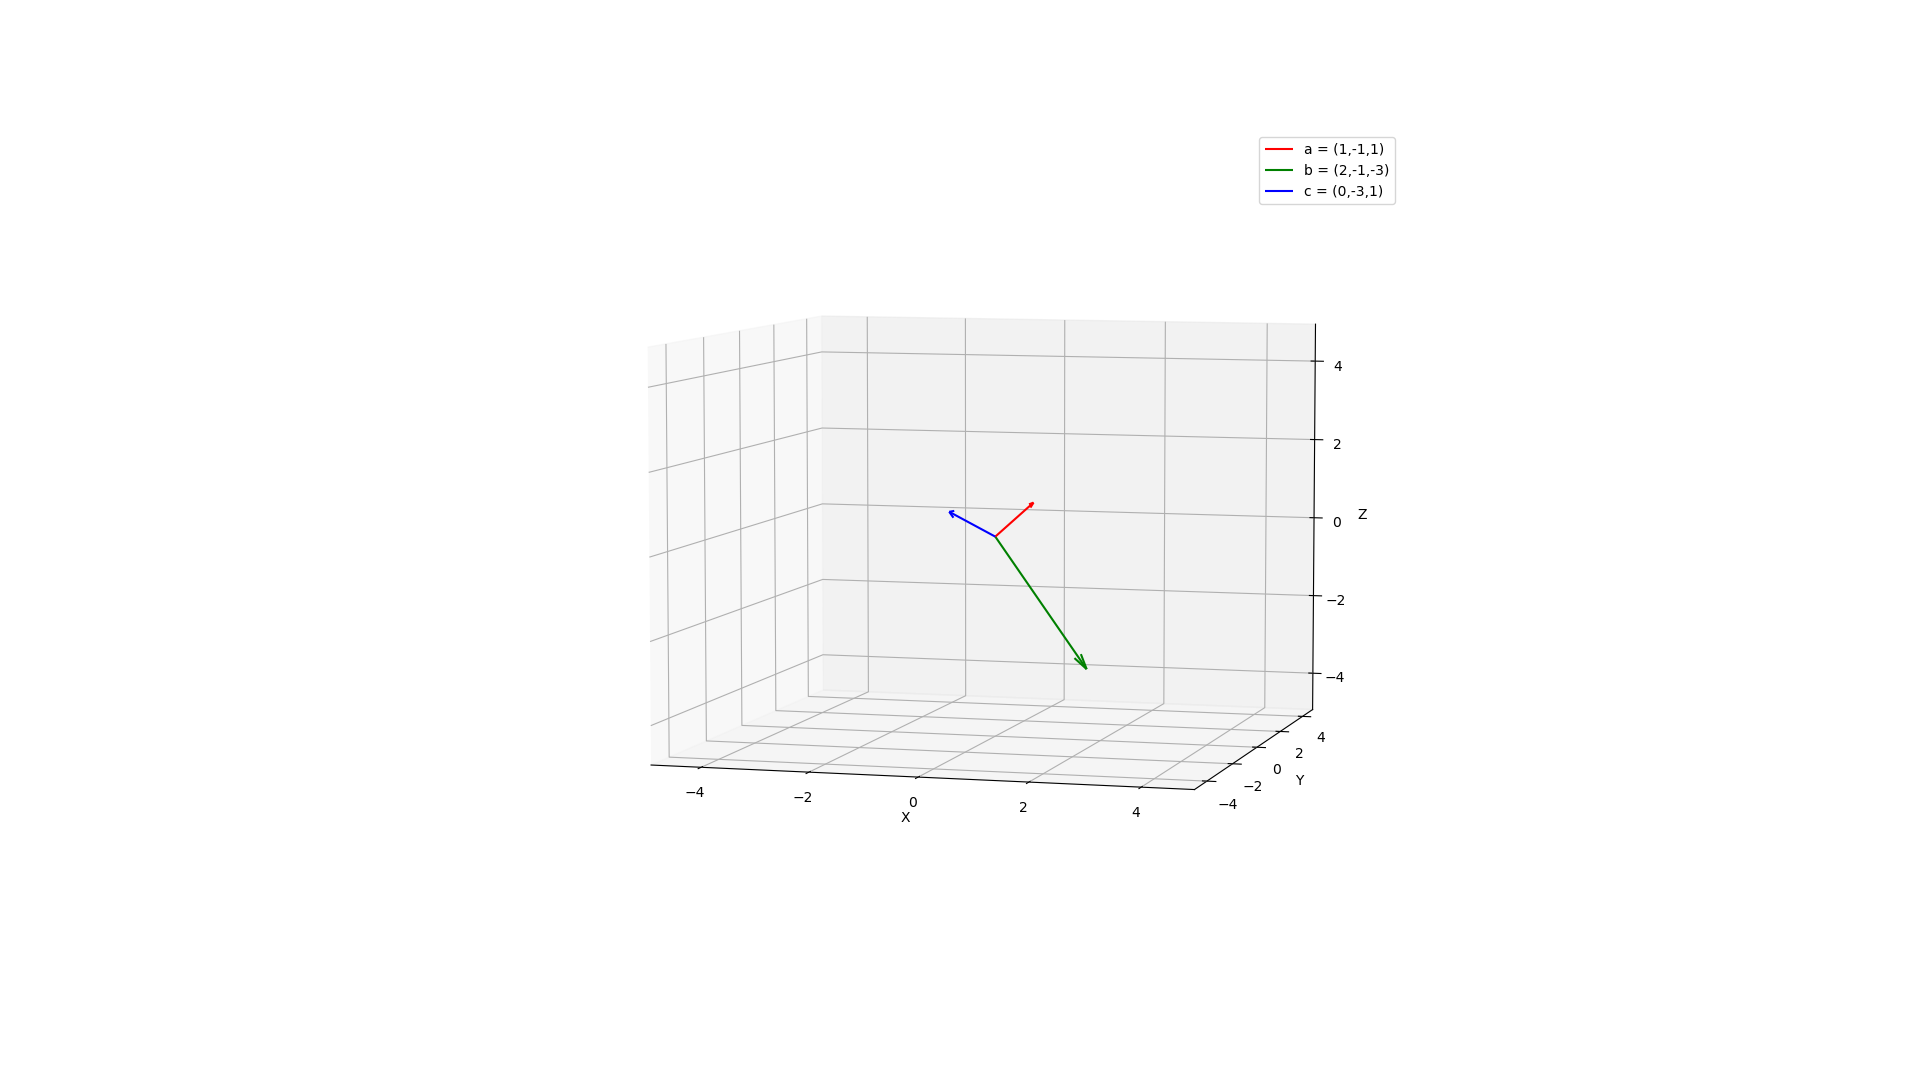
\includegraphics[width=1\columnwidth]{figs/plot4.png}
    \caption{}
    \label{fig:placeholder}
\end{figure}



\end{document}